%\documentclass[11pt, letterpaper, onecolumn]{article}
\documentclass{sig-alternate}

\usepackage{amsmath}
%\usepackage{times}
\usepackage{fullpage}
\usepackage{epsfig}
\usepackage{subfigure}
\usepackage{algorithm}
\usepackage{algorithmic}


\title{Space-Time Multiplexing of Stream Programs\vspace{-30pt}}

%\author{Michael Gordon, Jasper Lin, William Thies, and Saman Amarasinghe\\ \\
%  MIT Computer Science and Artificial Intelligence Laboratory\\
%  Cambridge, MA  02139\\ \\
%  \sffamily{\{mgordon, jasperln, thies, saman\}@cag.csail.mit.edu}}

% don't include the date
%\date{}

% this is the line spacing
%\setstretch{1.25}

% \sloppy lets Latex be a little less anal about interword spacing.  It is
% one way to eliminate those annoying Overfull hbox warnings.
% Another way is to surround each offending paragraph with
% \begin{sloppypar} ... \end{sloppypar}

%\sloppy

% See page 90 of the Latex book for info about vertical spacing probs.

\begin{document}

  \newcommand{\mt}[1]{\mbox{\it #1}}
  \newcommand{\todo}[1]{\framebox{#1}}

  %\toappear{\centerline{\Large\bf MIT LCS Technical Memo,}
  %          \centerline{\Large\bf MIT-LCS-TM-6XX,}
  %          \centerline{\Large\bf November, 2001.}}

\date{}  
\maketitle
\begin{abstract}
As DSP programming is becoming more complex, there is an increasing
need for high-level abstractions that can be efficiently compiled.
Toward this end, we present a set of aggressive optimizations that
target linear sections of a stream program.  Our input language is
StreamIt, which represents programs as a hierarchical graph of
autonomous filters.  A filter is linear if each of its outputs can be
represented as an affine combination of its inputs.  Linear filters
are common in DSP applications; examples include FIR filters,
expanders, compressors, FFTs and DCTs.

We present a linear extraction analysis that automatically detects
linear filters based on the C-like code in their {\tt work} function.
Once linear filters are identified, we show how neighboring nodes can
be collapsed into a single linear representation, thereby eliminating
many redundant computations.  Also, we describe a method for
automatically translating linear nodes into the frequency domain,
thereby yielding algorithmic savings for convolutional filters.

We have completed a fully-automatic implementation of the above
techniques as part of the StreamIt compiler, and we demonstrate
performance improvements that average 400\% over our benchmark
applications.




\end{abstract}
\vspace{-15pt}
\section{Introduction}

Applications that are structured around some notion of a ``stream''
are becoming increasingly important and widespread.  There is evidence
that streaming media applications are already consuming most of the
cycles on consumer machines \cite{Rix98}, and their use is continuing
to grow.  In the embedded domain, applications for hand-held
computers, cell phones, and DSP's are centered around a stream of
voice or video data.  The stream abstraction is also fundamental to
high-performance applications such as intelligent software routers,
cell phone base stations, and HDTV editing consoles.

Despite the prevalence of these applications, there is surprisingly
little language and compiler support for practical, large-scale stream
programming.  Of course, the notion of a stream as a programming
abstraction has been around for decades \cite{SICP}, and a number of
special-purpose stream languages have been designed (see
\cite{survey97} for a review).  Many of these languages and
representations are elegant and theoretically sound, but they often
lack features and are too inflexible to support straightforward
development of modern stream applications, or their implementations
are too inefficient to use in practice.  Consequently, most
programmers turn to general-purpose languages such as C or C++ to
implement stream programs.

There are two reasons that general-purpose languages are inadequate for
stream programming.  Firstly, they are a mismatch for the application
domain.  That is, they do not provide a natural or intuitive
representation of streams, thereby having a negative effect on
readability, robustness, and programmer productivity.  Moreover, because
the widespread parallelism and regular communication patterns of data
streams are left implicit in general-purpose languages, compilers are
not stream-conscious and do not perform stream-specific optimizations.
As a result, performance-critical loops are often hand-coded in a
low-level assembly language and must be re-implemented for each target
architecture.  This practice is labor-intensive, error-prone, and very
costly.

Secondly, general-purpose languages are a mismatch for the emerging
class of grid-based architectures \cite{smartmemories,rawshort,trips} that
are especially well-suited for stream processing.  Perhaps the primary
appeal of C is that it provides a ``common machine language'' for
von-Neumann architectures.  That is, it abstracts away the
idiosyncratic differences between machines, but encapsulates their
common properties: a single program counter, arithmetic operations,
and a monolithic memory.  However, for grid-based architectures, the
von-Neumann model no longer holds, as there are multiple instruction
streams and distributed memory banks.  Thus, C no longer serves as a
common machine language--in fact, it provides the wrong abstraction
for the underlying hardware, and architecture-specific directives are
often needed to obtain reasonable performance.  Again, this greatly
complicates the job of the programmer and hampers portability.

StreamIt is a language and compiler specifically designed for modern
stream programming.  The StreamIt language has two goals: first, to
provide high-level stream abstractions that improve programmer
productivity and program robustness within the streaming domain, and
second, to serve as a common machine language for grid-based
processors.  At the same time, the StreamIt compiler aims to perform
stream-specific optimizations to achieve the performance of an expert
programmer.

This paper motivates, describes, and justifies the high-level language
features of StreamIt, version 1.0.  The major limitation of StreamIt
1.0 is that all flow rates in the streams must be static; applications
such as compression that have dynamically varying flow rates will be
the subject of future work.  A large set of applications can be
implemented with static rates, and while dynamic rates will require a
different runtime model, it will still be essential to fully analyse
and optimize static sub-sections in order to obtain high performance.

The paper is organized as follows. In Section {\ref{sec:domain}}, we
characterize the domain of streaming programs that motivates the
design of StreamIt, and in Section~\ref{sec:overview} we describe the
language features in detail.  We present an in-depth example of a
software radio in Section~\ref{sec:example}, preliminary results in
Section~\ref{sec:results}, related work in Section~\ref{sec:related},
and conclusions in Section~\ref{sec:conc}.

  
%\begin{figure}[t]
%\eightpoint
%\begin{Verbatim}[numbers = left]
%int->int filter AssignPictureType(int width, 
%        int height, 
%        int numpictures) {
%    int frameno;
%
%    init {
%        frameno = 0;
%    }
%
%    work pop (width*height*3) push 2 {
%        push(frameno);
%        for (int i = 0; i < width*height*3; i++) {
%            pop();
%        }
%
%        int pushval;
%        int framecount = frameno % 12;
%        if (framecount == 0) {
%            pushval = 1;
%        } else if (framecount == 3 
%                || framecount == 6 
%                || framecount == 9) {
%            pushval = 2;
%        } else {
%            pushval = 3;
%        }
%
%        if ((frameno == (numpictures-1)) 
%            && (pushval == 3)) {
%            pushval = 2;
%        }
%
%        push(pushval);
%        frameno++;
%    }
%}
%\end{Verbatim}
%
%\caption{Example StreamIt program with AssignPictureType filter, used in MPEG Encoder.\protect\label{fig:apt-pipeline}}
%\end{figure}

\section{The StreamIt Language}
\label{sec:streamit}

StreamIt is an architecture-independent language for high-performance
stream programming~\cite{thies-cc02}.  The compiler is publicly
available~\cite{streamitweb} and includes backends for multicore
architectures, clusters of workstations, and Tilera architectures.

The model of computation in StreamIt is grounded in (but not limited
to) synchronous dataflow~\cite{lee87}.  In this model, the programmer
implements independent actors, or {\it filters}, which translate data
items from input channels to output channels.  Filters are composed
into graphs that represent the overall computation.  The key property
of synchronous dataflow is that the number of items consumed and
produced during each execution of a filter is known at compile time,
allowing the compiler to perform static scheduling and optimization.

An example StreamIt filter appears in Figure~\ref{fig:apt-pipeline}.
It is based on the AssignPictureType filter in the MPEG2 encoder.
StreamIt filters contain three stages of execution.  The most
important is the \work function, which represents the
steady-state execution step and is called repeatedly by the runtime
system.  Within the \work function, a filter may {\it peek} at a given
element on the input tape, {\it pop} an item off the input tape, or
{\it push} an item to the output tape.  The total number of items
peeked, popped, and pushed are declared as part of the \work function.
Note that if the peek rate exceeds the pop rate, it represents a
sliding window computation in which some input elements are accessed
across multiple invocations of the filter.

In addition to the \work function, a filter may declare an {\tt init}
function to initialize internal data structures, as well as a 
 \prework function (not given in Figure~\ref{fig:apt-pipeline}) to
perform specialized processing of data items prior to the steady
state.  The \prework function is needed in cases where the initial
processing has a different input or output rate than the steady-state
processing.

A {\it schedule} gives a multiplicity for each filter in a stream
graph.  The multiplicity indicates how often a filter's \work function
should be invoked (or \prework function on the first iteration of the filter).  The
{\it steady-state schedule} can be calculated such that all filters
fire in the schedule, and the schedule can be repeated
indefinitely~\cite{lee87}.  Steady-state execution of the graph
entails repeating the steady-state schedule for as much input as is
expected.  Execution of the stream graph is conceptually wrapped in an
outer loop that continuously executes the steady-state schedule.  All
the multiplicities of the steady-state can be multiplied by the same
constant $m$, and the result will still be a valid steady-state.  We
call this process {\it increasing} the steady-state of the graph by
$m$.

Furthermore, an {\it initialization} schedule enables the steady-state
schedule in the presence of peeking filters.  An initialization
schedule is required if peeking is present in a graph to enable the
calculation and execution of a steady-state
schedule~\cite{karczmarek-lctes03}.  During application execution, the
{\it init} function is called once for each filter, then the
initialization schedule is executed once, followed by an infinite
repetition of the steady-state schedule.

As depicted in Figure~\ref{fig:structures}, StreamIt provides three
hierarchical primitives for composing filters into stream graphs.  A
{\it pipeline} represents a sequential composition of streams, in
which the output of one stream feeds into the input of the next.  A
{\it splitjoin} represents a parallel set of streams, which divulge
from a common {\it splitter} and converge to a common {\it joiner}.
The types of splitters and joiners are predefined by the StreamIt
language; they encompass duplication and weighted round-robin
behaviors.  Finally, a {\it feedbackloop} represents a cycle in the
stream graph.

\begin{figure}[t!]
\centering
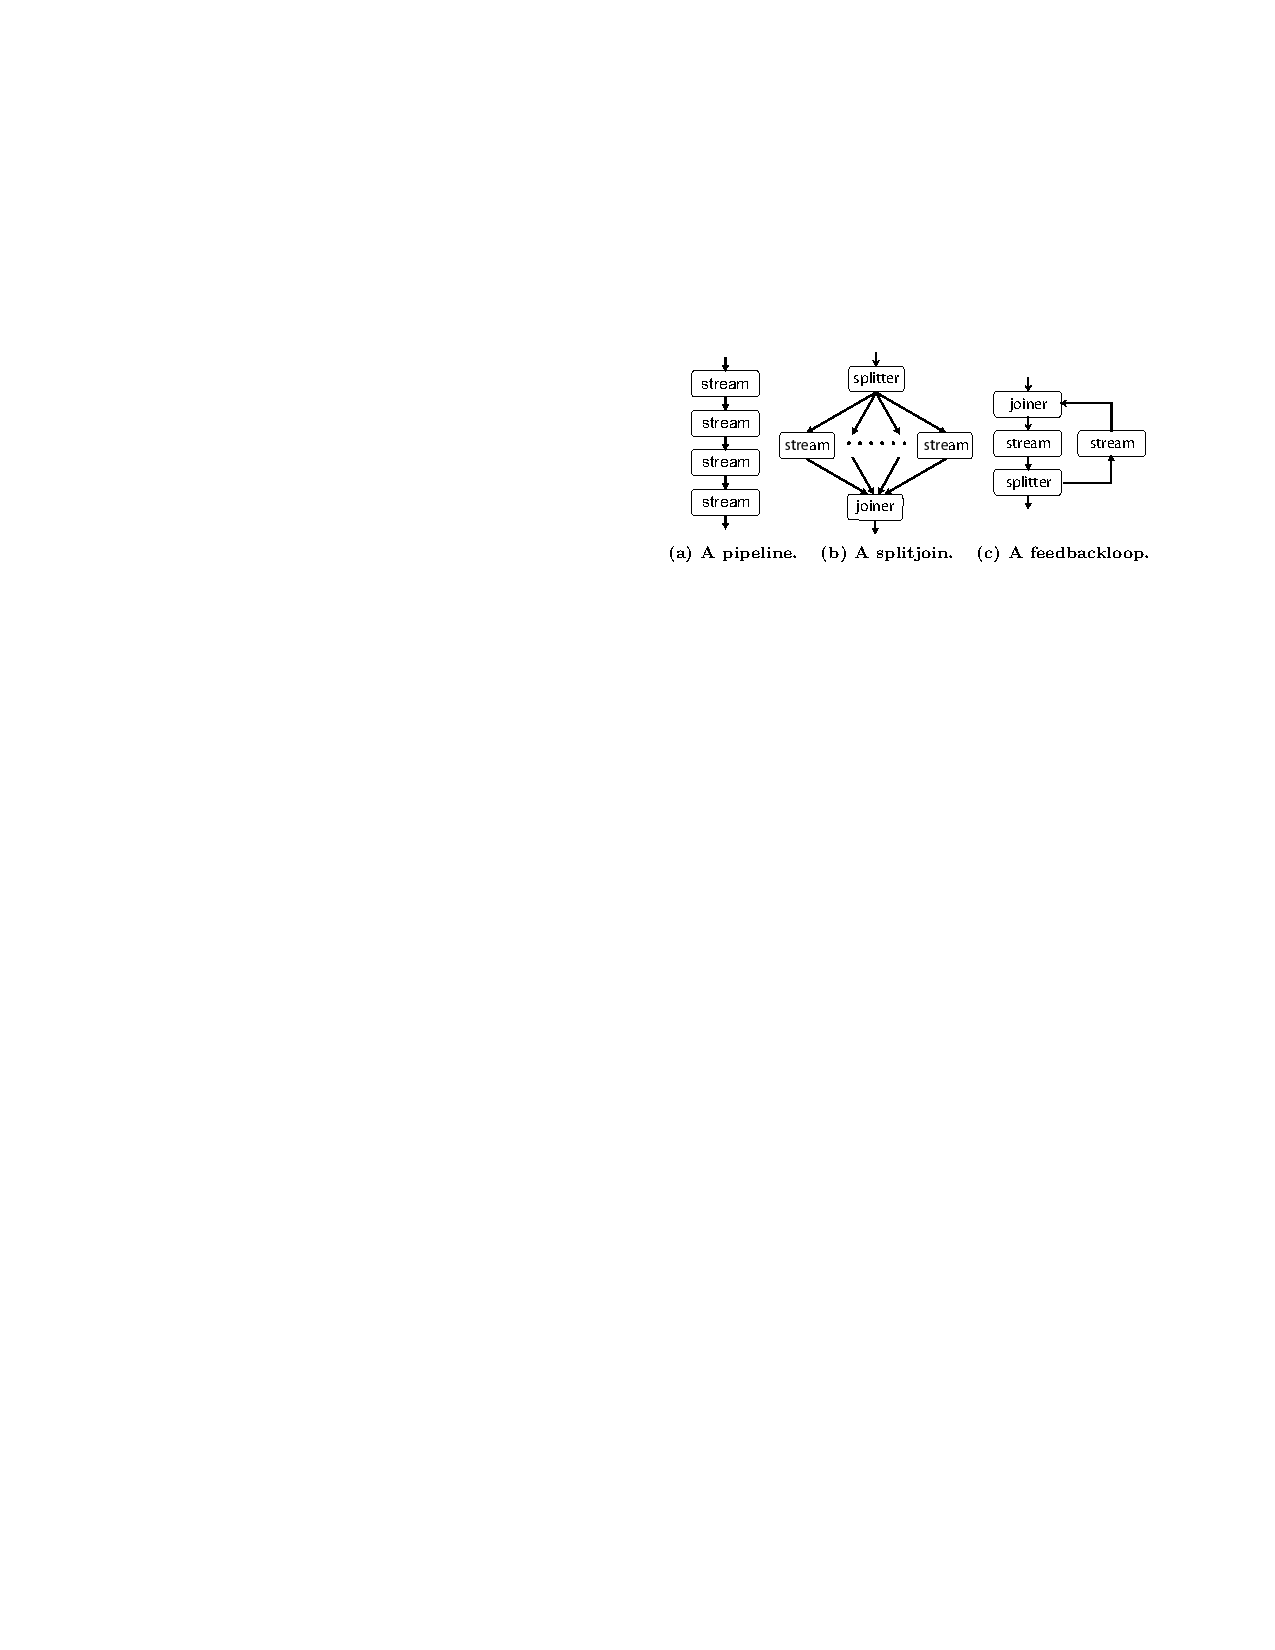
\includegraphics[width=3.3in]{stream-structures.pdf}
%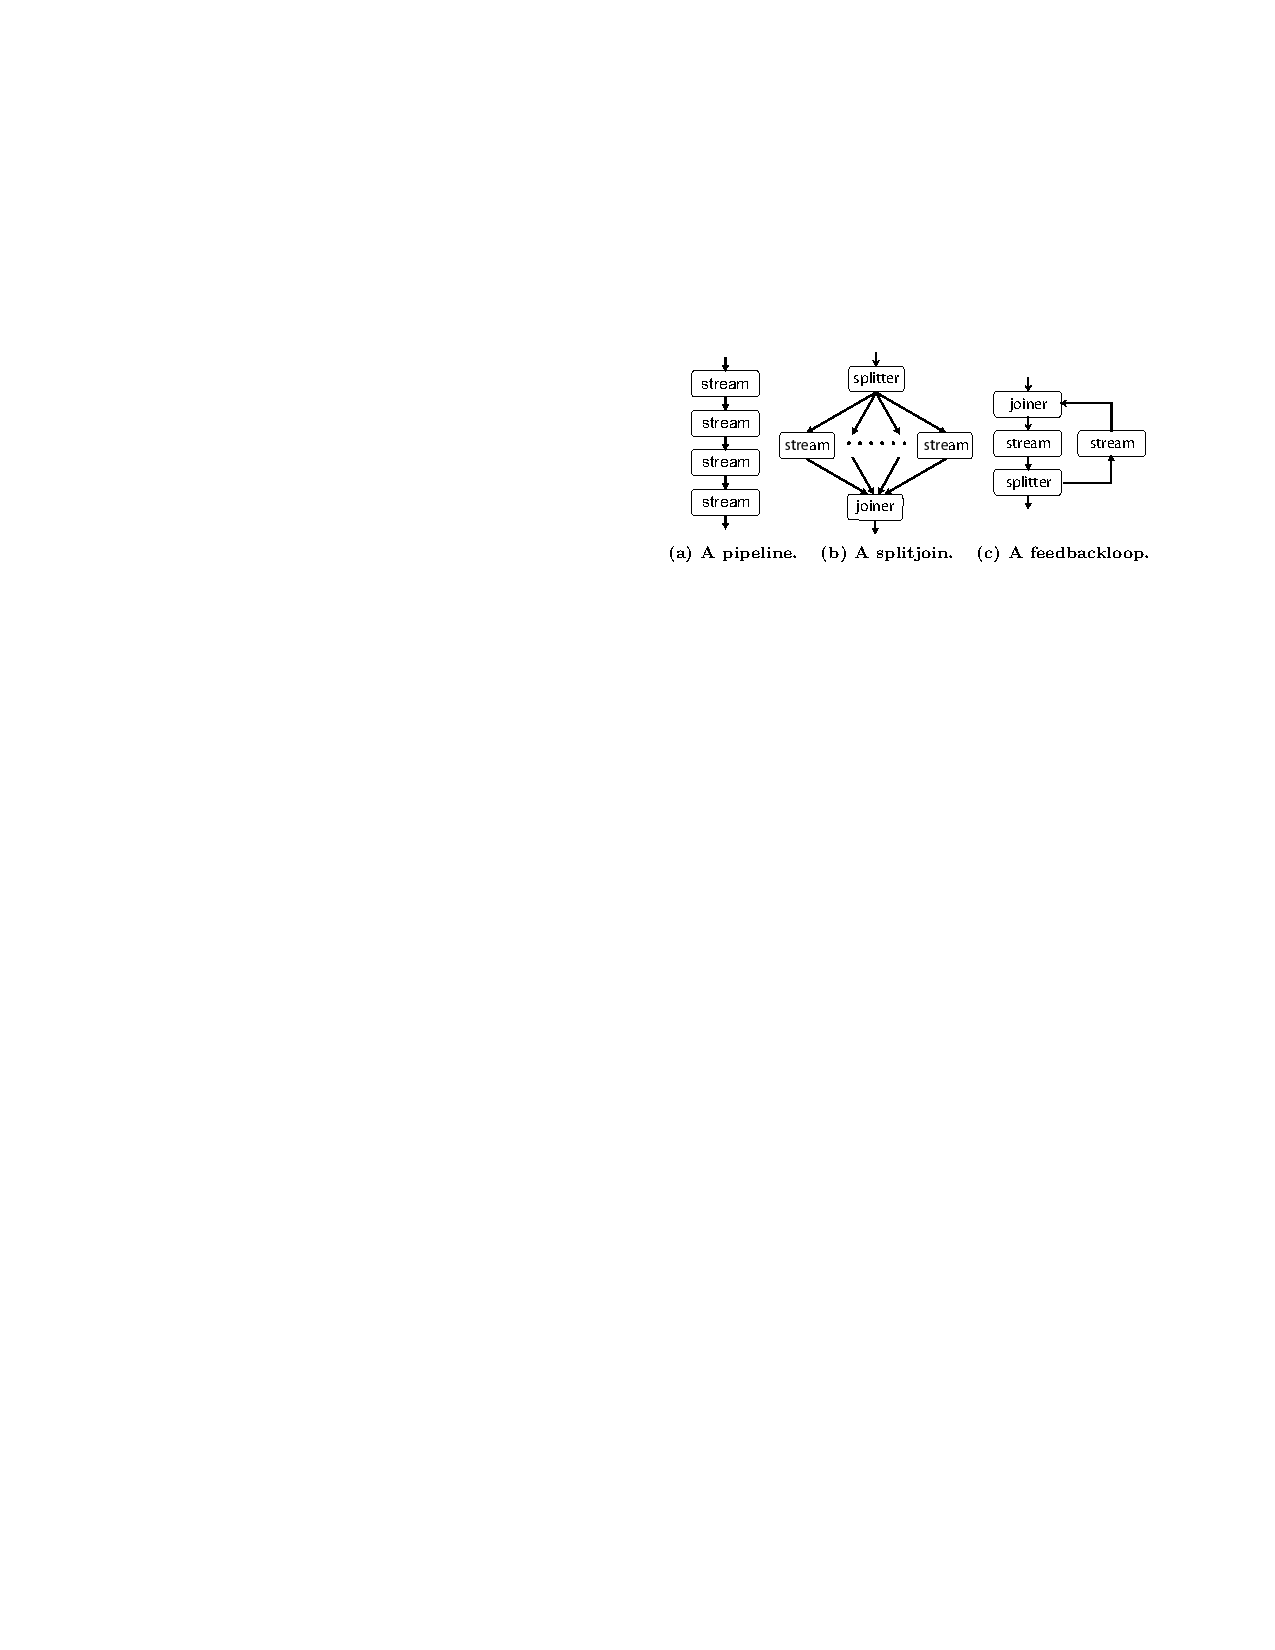
\psfig{file=stream-structures,width=\columnwidth}
\caption{Hierarchical stream structures supported by StreamIt.\protect\label{fig:structures}}
\end{figure}

The StreamIt compiler coarsens the granularity of a stream graph by
applying the {\it fusion} transformation which merges adjacent filters
into a single (large) filter (embedding the schedules of execution in
the merged filter)~\cite{streamit-asplos}.  The {\it fission}
transformation is employed to add data parallelism to a stream graph.
In fission, a single filter without state is duplicated a certain
number of ways and placed in a splitjion construct.  Input items to
the original filter are distributed among the duplicates, termed {\it
  fission products}.  In \S\ref{sec:fission}, we describe how to
extend the fundamental fission transformation to parallelize induction
variable state.
	
\begin{figure*}[th]
\vspace{-12pt}
\begin{minipage}{3.2in}
\begin{center}
\begin{minipage}{0.46in}
\centering
\psfig{figure=pipeline.eps,width=0.46in} \\
\end{minipage} 
~
\begin{minipage}{1.3in}
\centering
\psfig{figure=splitjoin.eps,width=1.3in} \\
\end{minipage}
~
\begin{minipage}{1.02in}
\centering
\psfig{figure=feedback.eps,width=1.02in} \\
\end{minipage} 
\\ ~ \\ {\protect\small (a) A pipeline. ~~(b) A splitjoin. ~~(c) A feedbackloop.}
\caption{Stream structures supported by StreamIt.
\protect\label{fig:structures}}
\end{center}
\end{minipage}
~~~~~
\begin{minipage}{3in}
\centering
\vspace{15pt}
\psfig{figure=raw-diagram.eps,width=3in}
\caption{Block diagram of the Raw architecture.
\protect\label{fig:raw-diagram}}
\end{minipage}
\vspace{-12pt}
\end{figure*}

\section{The Raw Architecture}
\label{sec:raw}

The Raw Microprocessor \cite{raw10,raw} addresses the wire delay
problem \cite{raw13} by providing direct instruction set architecture
(ISA) analogs to three underlying physical resources of the processor:
gates, wires and pins. Because ISA primitives exist for these
resources, a compiler such as StreamIt has direct control over both
the computation and the communication of values between the functional
units of the microprocessor, as well as across the pins of the
processor.

The architecture exposes the gate resources as a scalable 2-D array of
identical, programmable tiles, that are connected to their immediate
neighbors by four on-chip networks.  Values routed through the
networks off of the side of the array appear on the pins, and values
placed on the pins by external devices (wide-word A/Ds, DRAMS, etc.)
appear on the networks.  Each of the tiles contains a compute
processor, some memory and two types of routers--one static, one
dynamic--that control the flow of data over the networks as well as
into the compute processor (see Figure \ref{fig:raw-diagram}).  The
compute processor interfaces to the network through a bypassed,
register-mapped interface \cite{raw10} that allows instructions to use
the networks and the register files interchangeably.

Each tile's static router has a virtualized instruction memory to
control the crossbars of the two static networks. Collectively, the
static routers can reconfigure the communication pattern across these
networks every cycle.  The input and output possibilities for each
crossbar are: North, East, South, West, Processor, to the other
crossbar, and into the static router. The FIFOs are typically four or
eight elements large.  To route a word from one tile to another, the
compiler inserts a route instruction on every intermediate static
router.  Because the routers are pipelined and compile-time scheduled,
they can deliver a value from the ALU of one tile to the ALU of a
neighboring tile in 3 cycles, or more generally, 2+N cycles for an
inter-tile distance of N hops.

Because we generate regular bulk DRAM transfers, we did not want
accesses to off-chip memory to become the bottleneck of the hardware
configuration.  So, we use a simulation of a CL2 PC 3500 DDR DRAM,
which provides enough bandwidth to saturate both directions of a Raw
port \cite{raw_isca}.  In our configuration, we use 16 such DRAMs,
attached to each of the 16 logical ports of the chip.  Also, we
implemented a streaming memory controller in the chipset that supports
a number of simple streaming memory requests.  The chipset receives
request messages over the general dynamic network for bulk transfers
to and from the DRAMs.  The transfers themselves can use either the
static network or the general dynamic network (the desired network is
encoded in the request).  Simple interleaving and striding is
supported by the chipset, but is unused by the Spacetime Compiler,
since all DRAM accesses are to or from a contiguous chuck of memory
with unit stride. The chipsets also have a simple demultiplexing
mechanism that allows multiple devices (such as external input and
output streams) to share a single port.

The results of this paper were generated using btl, a cycle-accurate
simulator that models arrays of Raw tiles identical to those in the
.15 micron 16-tile Raw prototype ASIC chip.  With a target clock rate
of 450 MHz, the tile employs as compute processor an 8-stage, single
issue, in-order MIPS-style pipeline that has a 32 KB data cache, 32 KB
of instruction memory, and 64 KB of static router memory.

(FileReaders and writers should be talked about as connected to the
bypass port of the dram chipset).
\section{Stream Graph} 

\begin{figure*}
\centering
\psfig{figure=fm_example.eps,width=6.5in}
\caption{FMRadio with a 12-way equalizer after the passes of the
SpaceTime Compiler.
\protect\label{fig:fm-ex}}
\end{figure*}

Currently we use the StreamIt Programming Language as the input
language to the SpaceTime Compiler. After the StreamIt frontend
executes, it passes our compiler a complete stream graph representing
the computation and communication of the application.  In StreamIt,
the stream graph is a structured, hierarchical composition of
pipelines, splitjoins, and feedbackloops with filters, splitters, and
joiners as the leaf nodes of the graph (see Section
\ref{sec:streamit}).  

Throughout the following sections, we will use our FMRadio benchmark
to elucidate our discussion.  The FMRadio application is a software
implementation of FM radio with a 12-way equalizer.  StreamIt's stream
graph is given in Figure \ref{fig:fm-ex}a.  In the figure, we
represent splitters, joiners, and filters with circles.  Containers
(splitjoins and pipelines) are represented with as rectangles around
the nodes they contain.  In the figure, the filters colored red have
the highest work estimation per steady-state execution (in this case,
the red nodes account for over 90\% of the computation in the
steady-state).

The initial pass of our compiler takes this structured stream graph
and de-structures it.  We remove all hierarchy and structure of the
containers and are left with only filters, splitters and joiners.
Furthermore, we introduce our own notion of a splitter and a joiner,
each slightly more powerful than their analog in StreamIt.  We still
have separate nodes for splitting an output stream and joining an
input stream, but these nodes can handle more complicated
data-reorganization patterns.  For example, our splitter node can
describe a round-robin distribution with duplication.  A more exact
discussion of our splitters and joiners is omitted, but it suffices to
say that we designed each node to closely match the data-organizations
that are possible with a scalar operand network \cite{scalaroperands}.
We next run a synchronization removal pass that converts StreamIt
splitters and joiners into our own notion of data-distribution nodes.
In the process we remove unnecessary synchronization points present in
the stream graph.  We introduce a (more powerful) splitter node after
each filter whose output is read by multiple filters and we introduce
a (more powerful) joiner node before each filter that reads data
produced by multiple filters.

After synchronization removal, we are left with a flat stream graph
composed of filters, and data-reorganization nodes (our more powerful
splitters and joiners), see Figure \ref{fig:fm-ex}b FMRadio's
flattened stream graph; note that some splitters have been
coalesced. For the remainder of this paper the terms splitter and
joiner refer to our more powerful splitting and joining nodes and the
term stream graph refers to the flattened graph composed of these
nodes and filters.  At this point we are ready to extract the slices
from the graph and schedule them for execution.


\section{The Slice}

What is a slice?
Why a slice? (slight rehash of intro).
Restrictions.
Representation in the compiler.

\section{Model of Computation}
\label{model}

The model of computation employed for this paper is a general model
that is agnostic of input language.  The semantics of the model are
built upon synchronous dataflow (SDF)~\cite{leeSDF}.  Although
inspired by the StreamIt programming language, the model can represent
aspects of other streaming languages such as Brook~\cite{brook04},
Lime~\cite{lime10}, SPL~\cite{spl09} and SPUR~\cite{spur05samos}.
Consider a directed graph $G = (V, E)$ corresponding to a streaming
application. $F \in V$ is a filter in the application and $(f, g) \in
E$ is an edge (or {\it channel}) in the graph that denotes
communication from $f$ to $g$ using a FIFO channel.  Each filter is
described by rate declarations, data reorganization patterns,
and compute functions as described below. The techniques in this paper
require static-rate graphs, i.e., all of the quantities of the filters
are statically determinable.

%  Figure~\ref{fig:streamgraph} gives an example
% stream graph for a FM radio with an equalizer.  The figure also
% includes details for two of the filters; the details are explained
% below.

% The filter is the basic unit of execution in our model.  Each filter
% is described by multiple rate declarations, data reorganization
% patterns, and compute functions.  Basically, each filter defines the
% number of items it consumers and produces each time it is executed.
% The execution of a stream graph is represented by a {\it schedule} of
% a graph $G$.  A schedule gives a multiplicity for each filter $F \in
% V$ that denotes how many times to fire filter $F$.  When a schedule is
% executed, each filter fires when it has buffered enough input to
% satisfy its input requirement (a filter will not fire more times than
% given by a schedule).  In our notation, a schedule is represented by
% the variable $\Sigma$, and it denotes a mapping from filters to
% non-negative integers. The multiplicity of filter $F$ in schedule
% $\Sigma$ is denoted by $M(\Sigma, F)$.

For each filter, $F \in V$, a {\it work} function, $W_F$, is defined.
The work function defines the atomic execution step for each filter.
For each filter, $F \in V$, a {\it prework} function, $W_F^P$, can
also be defined.  Prework describes a computation step that executes
once at the first firing of a filter.  The prework function is
executed only once per execution of the {\it application}; it
describes any special initialization behavior required for a
filter. We denote a function with the variable $\mathcal{F} \in \{W^p,
W\}$.  We sometimes leave out the subscript that denotes the filter if
it is clear which work or prework function is intended.

For each filter $F \in V$ we define the following:
\begin{itemize}

\item $o(\mathcal{F}, F)$, or {\it pop} rate, is the number of items
  dequeued from $F$'s input buffer per firing of $\mathcal{F}$.

\item $e(\mathcal{F}, F)$, or  {\it peek} rate, 1 $+$ the greatest index that is read (but
  not necessarily dequeued) from $F$'s input buffer per firing of
  $\mathcal{F}$. 

\item $u(\mathcal{F}, F)$, or {\it push} rate , the number of items enqueued to $F$'s
output buffer per firing of $\mathcal{F}$.  

\end{itemize}

\noindent Sliding window filters have a peek rate greater than the pop
rate.  We somethings refer to sliding window filters as {\it peeking}
filters. Figure~\ref{fig:pipeline-example}(a)
demonstrates a peeking filter.  The figures shows that the window of
items read for 3 consecutive firings of the filter overlap.  For the
work function execution, a peeking filter $F$ requires $e(W_F, F)$
items to be on its input channel(s) to fire.  $F$ will consume
(dequeue) the first $o(W_F, F)$ items after the firing of the work function.

\begin{figure}[t]
\centering
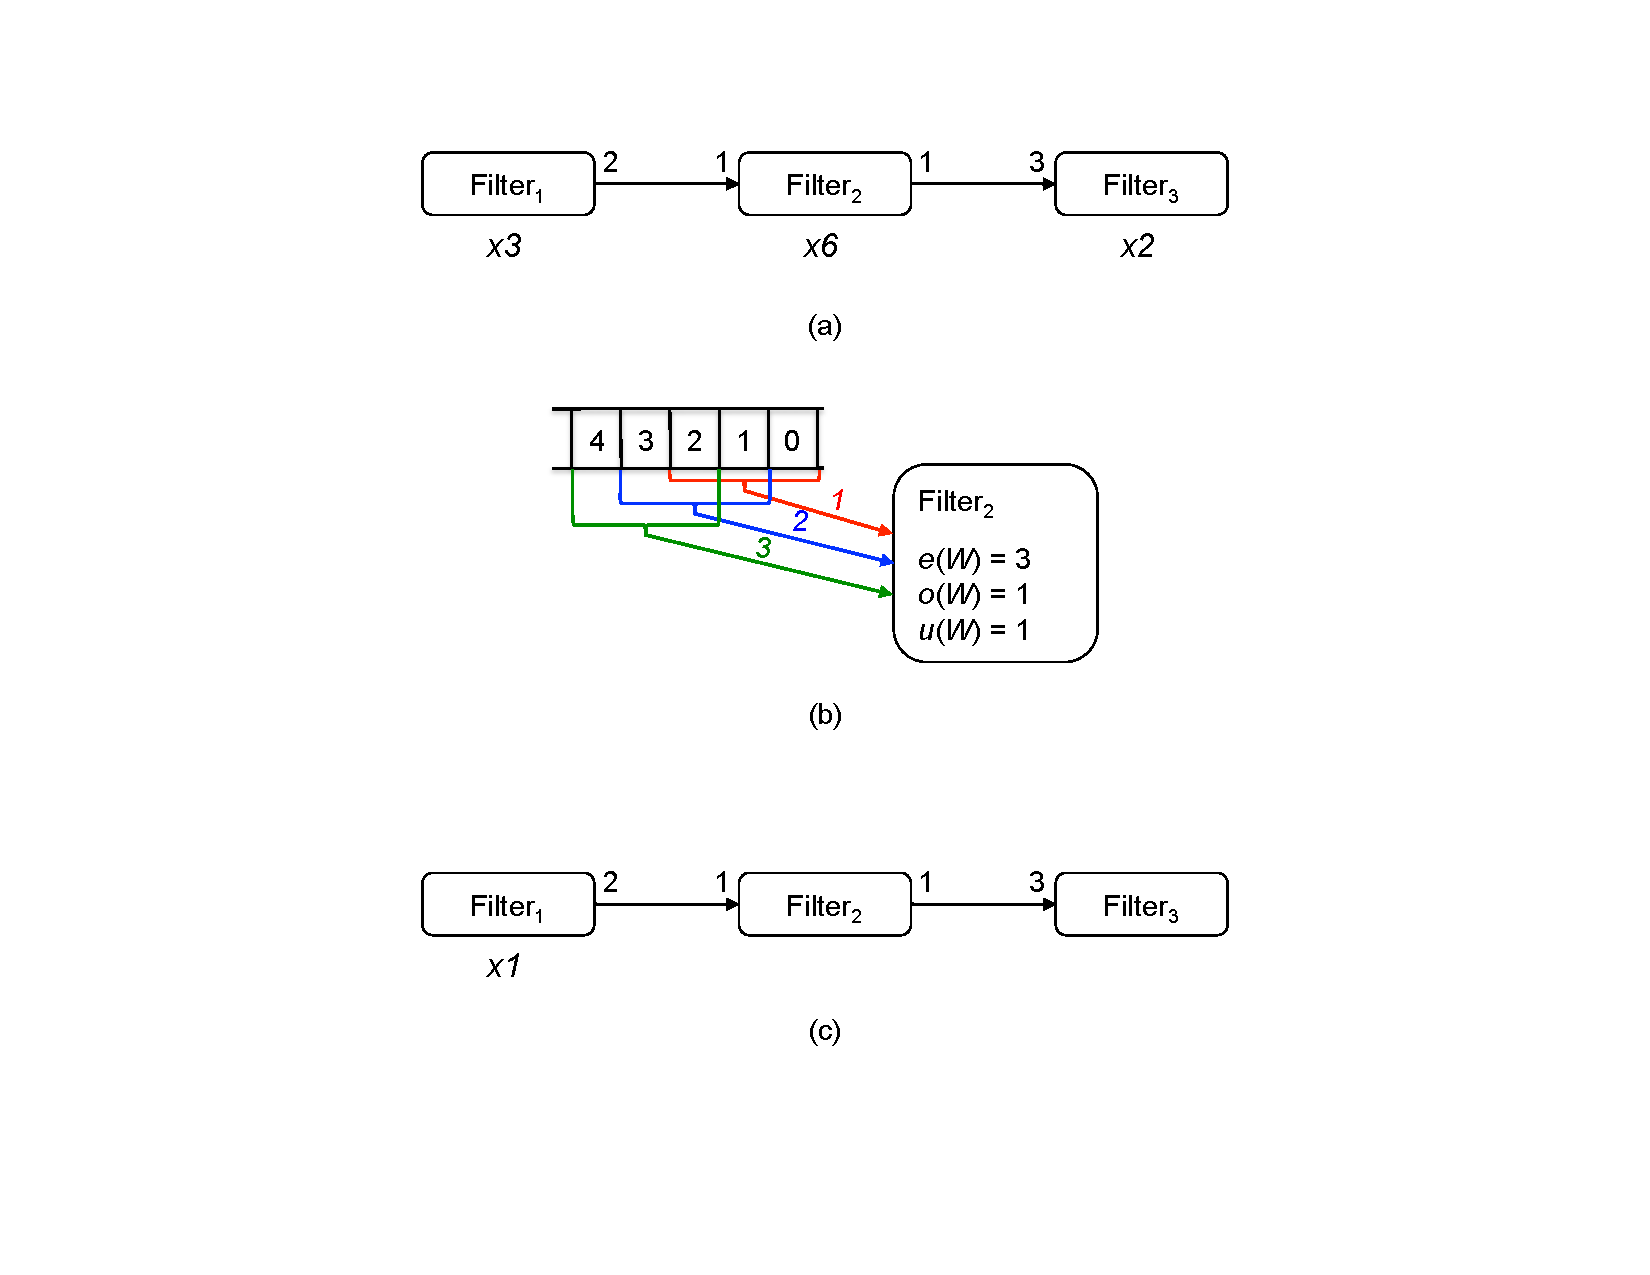
\includegraphics[width=3.0in]{figures/pipeline-example.pdf}
\caption[A pipeline of three filters with schedules.]{ (a) gives
  details for a sliding window filter.  The figure
  shows the window of items read for 3 consecutive firings of the
  filter.  Notice the overlapping in the windows.  (b) presents a pipeline of
  three filters with push and pop rates.  (b) also gives a
  legal steady-state schedule and initialization schedule for the
  three filters. $C(\mt{Filter}_2) = 2$ and
$C(\mt{Filter}_1) = C(\mt{Filter}_3) = 0$. 
  \label{fig:pipeline-example}}
\vspace{-10pt}
\end{figure}

A schedule gives a multiplicity for each filter $F \in V$ that denotes
how many times to fire filter $F$. A {\it steady-state schedule} can
be calculated such that all filters fire in the schedule, and the
schedule can be repeated indefinitely~\cite{lee87}.  Steady-state
execution of the graph entails repeating the steady-state schedule for
as much input as is expected.  Execution of the stream graph is
conceptually wrapped in an outer loop that continuously executes the
steady-state schedule.  Figure~\ref{fig:pipeline-example}(b) gives an
example of a steady-state schedule calculated for a graph that
consists of three filters in a pipeline.  All the multiplicities of
the steady-state can be multiplied by the same constant $c$, and the
result will still be a valid steady-state.  We call this process {\it
  increasing} the steady-state of the graph by $c$.

Our model does not deal with arbitrary schedules of filter executions.
The steady-state schedule, $S$, is explicitly represented.
Furthermore, an {\it initialization} schedule, $I$, is explicitly
represented that enables the steady-state schedule in the presence of
peeking filters.  An initialization schedule is required if peeking is
present in a graph to enable the calculation and execution of a
steady-state schedule~\cite{karczmarek-lctes03}.  After the initialization
schedule executes, each filter $F$ is guaranteed to have at least
$e(W_F, F) - o(W_F, F)$ items in its input buffer.
Figure~\ref{fig:pipeline-example}(b) gives a legal initialization
schedule for the pipeline that enables the peeking in filter
$\mt{Filter}_2$.  During application execution, the initialization
schedule is executed once followed by an infinite repetition of the
steady-state schedule.  The number of items remaining on $F$'s input
channel(s) after execution of the initialization schedule is
represented by $C(F)$.

In our notation, a schedule is represented by the variable $\Sigma$,
and it denotes a mapping from filters to non-negative integers. In our
execution model, only an initialization schedule and a steady-state
schedule are considered (thus $\Sigma \in I,S$). The
multiplicity of filter $F$ in schedule $\Sigma$ is denoted by
$M(\Sigma, F)$.  

A filter may have multiple incoming edges and/or multiple outgoing
edges.  Filter inputs are organized into a single internal FIFO buffer for the
filter to read according to an {\it input distribution pattern}, and
filter outputs are distributed from a single internal output FIFO
buffer according to an {\it output distribution pattern}.   
The input distribution pattern is represented as:
{\ninepoint
\[ \mt{ID}(\Sigma, F) \in (\mathbb{N} \times E)^n = ((w_1,e_1), (w_2,
e_2), ..., (w_n, e_n))\]
}
\noindent Where $n$ is the width of the input distribution pattern.
The input distribution describes the round robin joining pattern for
organizing the input data into the filter's single internal FIFO
buffer, where $w_i$ items are received from edge $e_i$ before
proceeded to the next edge, $e_{i+i}$.

The output distribution pattern describes both round-robin
splitting and duplication in a single structure:
{\ninepoint
\[ \mt{OD}(\Sigma, F) \in (\mathbb{N} \times (P(E)-\emptyset))^m = ((w_1,d_1), (w_2,
d_2), ..., (w_n, d_n))\]
}
\noindent Where $P(E)$ is the powerset of $E$.  Each $d_i$ is called
the {\it dupset} of weight $i$.  The dupset $d_i$ specifies that $w_i$
items be duplicated to the edges of the dupset.  Each tuple denotes
that $w_i$ output items of $F$ are duplicated to the edges of $d_i$
before moving on to the next tuple.

\begin{figure}[t]
\centering
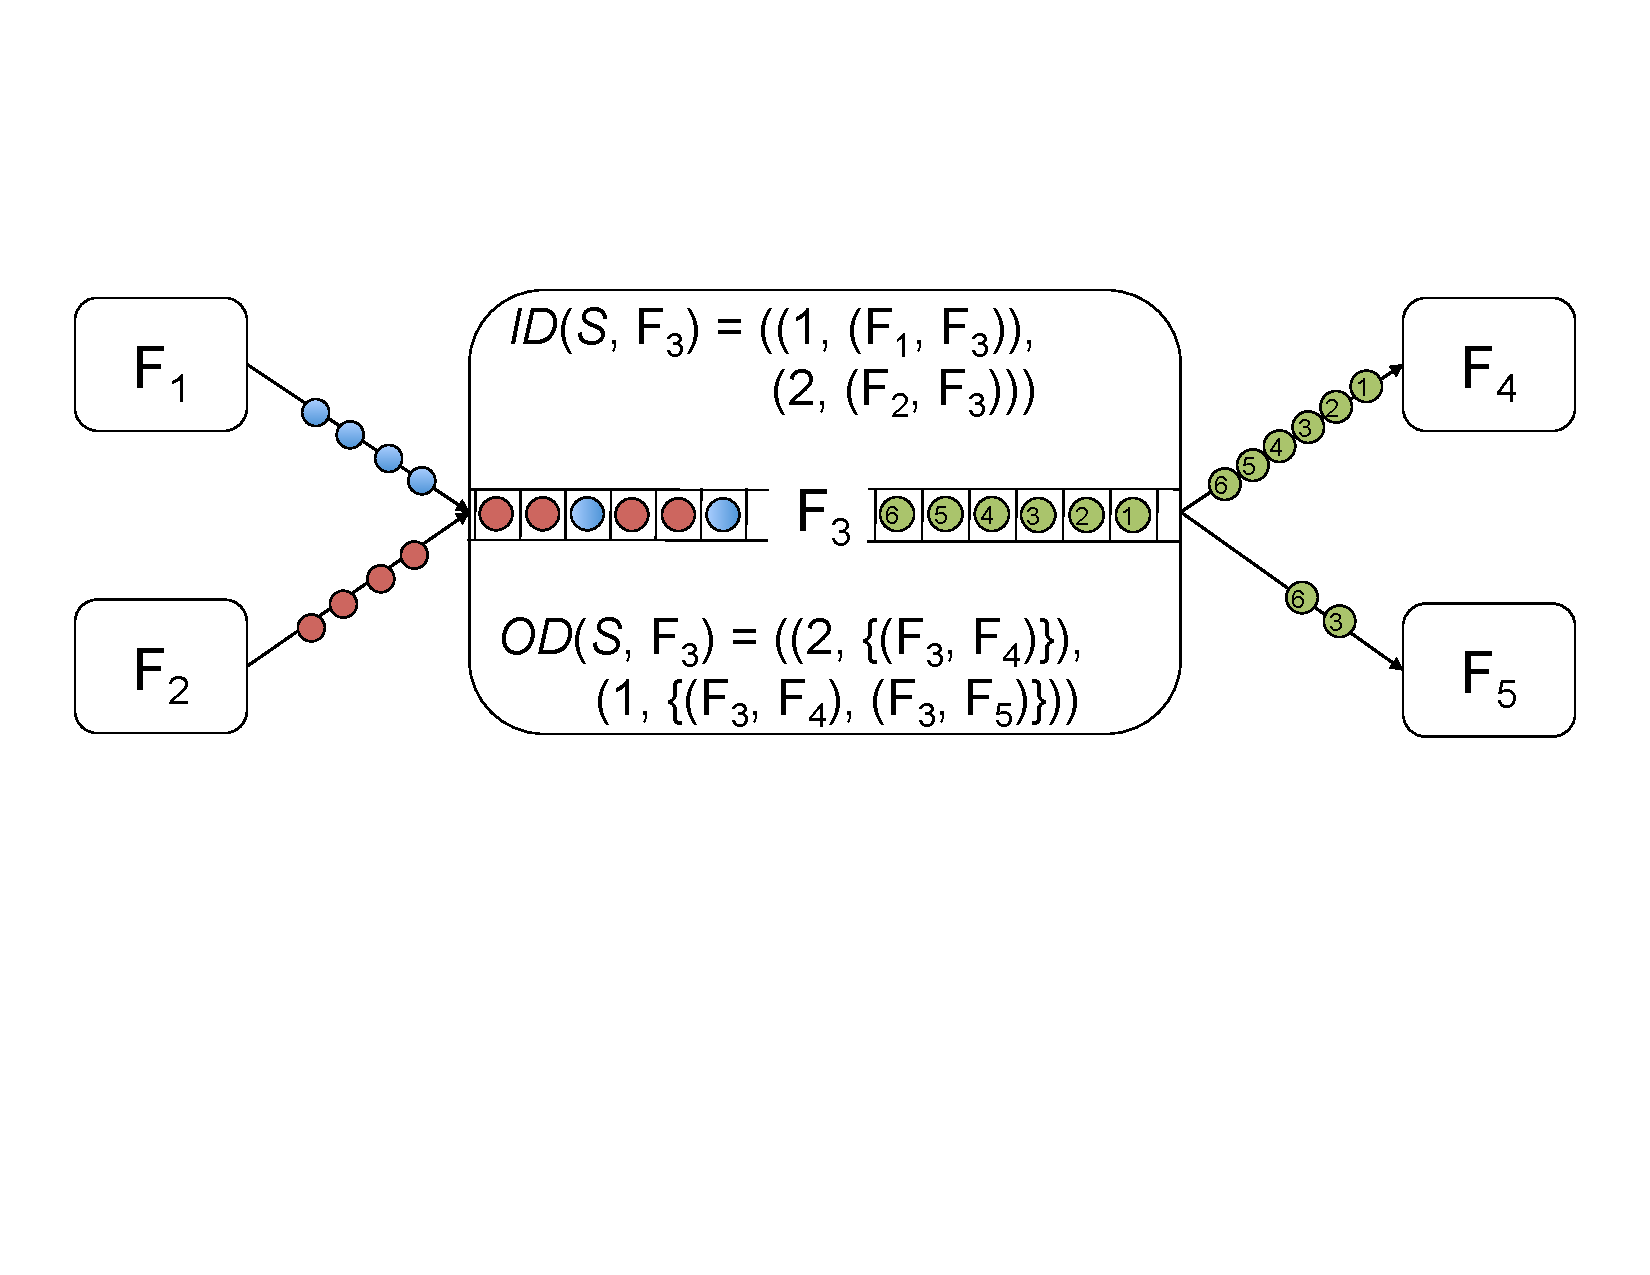
\includegraphics[width=3in]{figures/dist-example.pdf}
\caption[Example of input and output distribution.]{
An example of a filter with non-trivial input and output distribution patterns.
Filter $F_3$ has both multiple inputs and multiple outputs.  The input
items from the multiple inputs are joined in the pattern described by
its input distribution ($ID$): receive 1 item from $F_1$ and 2
items from $F_2$, and repeat.  $F_3$'s output items are distributed to
its multiple outputs as described by the output distribution pattern
($OD$):  2 items to $F_4$, then 1 item is duplicated to both $F_4$ and
$F_5$.  The output items of $F_3$ are indexed to show how they are
distributed to $F_4$ and $F_5$.
\label{fig:dist-example}}
\vspace{-10pt}
\end{figure}

The input and output distributions are repeated as needed for the
schedule that is being executed.  The start of each steady-state
iteration resets the input and output distributions to the first tuple.
Figure~\ref{fig:dist-example} highlights an example of a filter with
both multiple inputs and multiple outputs, and how the distribution
patterns translate into scattering and gathering.

Let $\mt{RO}(F_1, F_2, \Sigma)$ be the ratio of output items $F_1$
splits along the edge $(F_1, F_2)$ to the total number of items that
$F_1$ produces in the schedule $\Sigma$.  This can be calculated from
$F_1$'s output distribution pattern for $\Sigma$.  For example, in
Figure~\ref{fig:dist-example}, $\mt{RO}(F_3, F_4) = 1$ and
$\mt{RO}(F_3, F_5) = \frac{1}{3}$.  Conversely, let $\mt{RI}(F_1, F_2,
\Sigma)$ be the percentage of total input items that $F_2$ receives
from $F_1$ for $\Sigma$.  For example, in
Figure~\ref{fig:dist-example}, $\mt{RI}(F_2,F_3) = \frac{2}{3}$.

% Let $s(\mathcal{F}, F)$ denote the execution time (in cycles, with
% respect to a given real or conceptual machine) of function
% $\mathcal{F}$ of filter $F$.  For many of the static scheduling
% techniques covered in this thesis, we calculate a static estimation of
% the total amount of work for a filter $F$ in the steady-state, $s(W,
% F) \cdot M(S, F)$.  We often use the term {\it work estimation} to
% denote this quantity.

\section{Slice Extraction}

\begin{figure*}
\centering
\psfig{figure=fm_example.eps,width=4.5in}
\caption{FMRadio with a 7-way equalizer after the passes of the
SpaceTime Compiler.
\protect\label{fig:fm-ex}}
\end{figure*}

\label{sec:extract}
After the StreamIt frontend executes, it passes our compiler a
complete stream graph representing the computation and communication
of the application.  In StreamIt, the stream graph is a structured,
hierarchical composition of pipelines, splitjoins, and feedbackloops
with filters, splitters, and joiners as the leaf nodes of the graph
(see Section \ref{sec:streamit}).

We will use our FMRadio benchmark to elucidate our discussion.  The
FMRadio application is a software implementation of FM radio with a
7-way equalizer.  StreamIt's stream graph is given in Figure
\ref{fig:fm-ex}a.  In the figure, we represent splitters, joiners, and
filters with circles.  Containers (splitjoins and pipelines) are
represented as rectangles around the nodes they contain.  In the
figure, the filters colored red have the highest workload per
steady-state execution (in this case, the red nodes account for over
90\% of the computation in the steady-state).

The initial pass of our compiler takes this structured stream graph
and de-structures and canonicalizes it.  We remove all hierarchy and
structure of the containers and are left with only filters, splitters
and joiners. We are left with a flat stream graph composed of filters,
and data-reorganization nodes (splitters and joiners), see Figure
\ref{fig:fm-ex}b FMRadio's flattened stream graph; note that some
splitters have been coalesced.

Conceptually, the slice is the atomic unit of scheduling in our
compiler.  Our scheduling algorithm operates at the slice level.  Each
slice is composed of a contiguous region of the stream graph with
restrictions on its composition.  Slice extraction refers to the
process of assigning each joiner, filter, and splitter of the stream
graph to a slice.  As stated previously, a slice is a contiguous
section of the stream graph that is scheduled for execution as a
group. Each slice occupies a portion of the chip as it executes and is
``swapped out'' when it completes execution, not to execute again
until the next steady-state.  Each filter in the stream graph is a
member of exactly one slice.

We traverse the stream graph in depth-first order.  Each time we visit
a node, we must decide if the node should be added to the slice we are
currently constructing.  Due to the restrictions of the current
implementation, as we traverse the stream graph, we end the current
slice {\it before} a joiner node and we end the current slice {\it
after} a splitter node, thus restricting the slices to pipelines of
filters.  Also, as we are adding filters to the slice, we must
introduce a slice boundary if the size of the slice is equal to the
number of tiles in the Raw configuration.

Additionally, we try to coax the generation of load-balanced slices.
For each filter, we calculate a static work estimation of the filter
based on an analysis of the {\tt work} function
\cite{streamit-asplos}.  Because of the static I/O (push, pop, and
peek) rates in this version of StreamIt, most loop bounds within {\tt
work} can be resolved, allowing a close approximation of the actual
cycle count.  This estimate is multiplied by the number of times the
filter executes in the steady-state.

As we are adding filters to the slice, we compare the work estimation
of the current filter we are examining to the work estimation for the
filter of the slice that performs the most work (the current {\it
bottleneck} of the slice).  If the ratio of the work of the current
filter to the work of the bottleneck is within a predefined threshold,
termed the {\it work threshold}, then we proceed to add the filter to
the slice.  Otherwise, begin a new slice with the current filter as
the first filter in this new slice. In the case where a slice will end
in a filter, we will insert a dummy splitter at the end of the
just-completed slice.  Conversely, if needed, we will insert a dummy
joiner at the beginning of a newly created slice if the slice begins
with a filter. Any data-flow arcs that existed from splitters and to
joiners will persist as arcs to nodes of other slices.  The arcs of
the introduced splitters and joiners assume the connections of their
insertion point.

In Figure \ref{fig:fm-ex}c, we give a possible slice graph for the
7-way FMRadio application.  The blue boxes represent individual
slices.


\section{Space-Time Scheduling}
\label{sec:scheduling}
\subsection{Steady-State Schedule}

\begin{figure}
\centering
\psfig{figure=scheduling_2d.eps,width=3in}
\caption{The bin-packing, slice scheduling problem in two dimensions.
\protect\label{fig:2d}}
\end{figure}

what we get at this stage

3d bin packing translation

What the pieces look like 

saman's figures...

We arrive at a solution to the 3d bin packing by using simulated
annealing \cite{simanneal}, a type of iterative improvement.  A
detailed explanation of simulated annealing is beyond the scope of
this paper.  Simulated annealing is a form of stochastic
hill-climbing. Unlike most other methods for cost function
minimization, simulated annealing is suitable for problems where there
are many local minima.  Simulated annealing achieves its success by
allowing the system to go uphill with some probability as it searches
for the global minima.  As the simulation proceeds, the probability of
climbing uphill decreases.

talk about inter-trace-buffer assignment!

Calculate a total ordering of slices...

initial schedule is random

don't need to map the splitters and joiners, done by the static network.

mapping of tiles to drams.

How the solution creates the schedule...

\subsection{Cost Function}
The cost function for the simulated annealing solution to our 3D bin
packing problem attempts to incorporate three different aspects of the
scheduling problem.  First that the critical path of the schedule is
determined by the node(s) with the maximum work.  We do not generate a
true modulo schedule because all nodes must wait for the bottleneck
node to complete to perform the data-reorganization.  Next, we assume
that the work estimation performed by our compiler is inaccurate, so
we bias the estimate to reflect this observation.  Finally, we take
into account the communication cost of the data-reorganization phase.

As mentioned above, we would like to account for the intra-slice
pipeline startup and wind-down shape of the slices.  We would like the
slices of the final schedule to be placed like a Tetris-master would
align the falling pieces he or she encounters.  Toward this goal, our
node work estimation component of the cost function models these
properties.  Given an assignment of filters of the slices to nodes,
we arrive at the cost estimation for each tile using Algorithm
\ref{alg:tilework}. 

\begin{algorithm}
\caption{nodeWorkEst} \label{alg:tilework} {\tt
nodeWorkEst(}$T${\tt ,}$M${\tt )}. Given a the slice ordering $T$, and
$M$, a map of filters to computation nodes, return $C$, a map of nodes
to integers that represents the work of the node given the assignment $M$.
\begin{algorithmic}
\FORALL {$t \in T$}
\STATE Determined the  of 
\IF {$u$ scheduled before $t$ in $S$}
\STATE $u.prologue = t.prologue$
\ELSE
\STATE $u.prologue = t.prologue + 1$ 
\ENDIF 
\STATE {\tt incrementUpStream(}$u${\tt ,}$S${\tt )}
\ENDFOR
\end{algorithmic}
\end{algorithm}


link contention in the cost function
what it does!

\subsection{Prologue Schedule}
The prologue schedule guarantees that when the steady-state commences,
all the slices are ready to fire irrespective of their data-flow
dependencies.  To create this schedule we iteratively execute slices,
at each iteration we fire all the slices that can fire.  Stop the
schedule when all slices are ready to fire.

\subsection{Peek Initialization Schedule}
Before both the prologue schedule is executed and the steady-state
schedule is commenced, we perform a {\it peek initialization
schedule}.  This schedule is required to make sure that we can create
a cyclic steady-state schedule that respects StreamIt's peeking
operation.  In this schedule, slices are executed in data-flow order
and the buffers are not rotated.  Therefore, the prologue schedule
starts with the rotating buffers untouched.  See
\cite{streamitcc} for a more complete discussion of the peek
initialization schedule.



\section{Code Generation}
\label{sec:codegen}
In this section we consider low-level code generation for the Raw
microprocessor. Each Raw tile is an amalgam of the filters that
execute on it. To generate the execution code for the entire
application, we traverse the schedule for each phase of computation:
first the peek initialization stage, then prologue stage, and finally
the steady-state.  As we traverse each schedule, we generate the
computation and communication code as we visit each slice.  For the
initialization and prologue stages, we do a traversal of the slice
graph that respects the data-dependencies stipulated by the stream
graph. For the steady-state we traverse the schedule as calculated by
the slice scheduling algorithm of Section \ref{sec:scheduling}.

When we visit a slice, we first generate the DRAM requests and
communication code load its inputs from and store its outputs to its
mapped off-chip DRAM.  Next, we generate computation and communication
code for each filter of the slice.  

\subsection{Slice Data Reordering}
Before a steady-state execution can commence, each slice's single
input stream must be assembled in the order stipulated by the
round-robin weights on its incoming channels. To achieve this, the
various input streams of the slices are collected into the memory
module attached to the tile to which the first filter of the slice is
mapped. Streaming DRAM requests are generated to read each input
channel and to write the final, reassembled input.  Code is generated
for the static routers, as they perform the ordering of the final
input stream as stipulated by each joiner.  Splitting is done in much
the same way.  The compute processor of Raw are idle during
data-reorganization stage.

Remember from Section \ref{sec:softpipe} that the source and
destination buffers of this stage are the rotating buffers that
facilitate the software pipeline.  The number of individual memory
blocks that compose the rotating buffer is determined by the
multiplicity difference between the source slice and destination slice
in the prologue schedule.  Each time an off-chip memory request is
issued, the buffer will rotate, with two rotation structures for each
buffer that rotate separately, one for reading and one for writing.

\subsection{Filter Code Generation}
We generate computation and communication code for the individual
filters of the slice in much the same way as \cite{streamit-asplos}.  
%When we visit a slice in the schedule for each execution phase, we
%iterate over the filters that compose the slice, generating 
%communication and computation code necessary to execute the slice.
%The scheduling phase (Section \ref{sec:scheduling}) produces a mapping
%of filters to tiles.

%\subsubsection{Compute Processor}
%%For linear slices, we generate parameterized, template assembly code
%%for both computation and communication as described in Section
%%\ref{sec:linear}.  
%As we iterate over the filters of the slice, we append the code
%necessary to execute the current filter to the existing code for the
%tile to which the filter is mapped.  We also make sure to execute the
%{\tt init} function of each filter before we start the peek
%initialization stage. Consequently, each compute processor begins by
%calling the {\tt init} function of all the filters mapped to it.
%Next, the compute processor executes the {\tt work} function of each
%filter assigned to it in sequence.  The sequence is determined by the
%traversal of the schedule of each execution phase; first the
%peek initialization stage, then the prologue stage, and finally the
%steady-state.  Each work function execution is placed in a loop that
%executes the number of times the filter fires in the current stage.

%For Raw's compute processor, we generate a mixture of C code
%and assembly instructions that is compiled using Raw's GCC 3.3
%port. The translation of the {\tt init} function, {\tt work}
%functions, and any helper function is, for the large part,
%straightforward.  Most StreamIt expression have direct analogs in C
%except for the channel expressions {\tt push()}, {\tt peek(index)} and
%{\tt pop()}.

%One major benefit of StreamIt over other streaming languages is that
%the StreamIt compiler is responsible for buffer management.  The
%programmer is free to call {\tt pop()} or {\tt peek(index)} without
%having to worry about the structure of the buffer or updating the
%buffer's index variable after each execution of the work function.
%Currently, we classify filters as one of three types with respect to
%buffer management:
%\begin{enumerate}
%\item If a filter $(i)$ does not contain any {\tt peek} statements, $(ii)$
%does not contain any control-flow dependent channel expressions, and
%$(iii)$ has peek rate equals to pop rate, then a buffer is not needed
%and {\tt pop()} statements are translated directly into static network
%receives.  There exist other initialization considerations which are
%beyond the scope of this paper.
%\item If a filter contains peek statements, but $peek = pop$ then we can
%use a simple linear buffer that is reset after each work function execution.
%\item Otherwise, when $peek > pop$, we use a circular buffer to
%account for the data remaining on the channel after the work function
%invocation.
%\end{enumerate}
%Each {\tt push()} statement is translated directly into a static
%network send.  

%\subsubsection{Switch Processor}
%As mentioned in Section \ref{sec:implementation}, individual slices
%are limited to pipelines, thus we do not have to worry about
%complicated patterns for intra-slice communication.  For each tile we
%place the switch instructions to receive $pop$ items from the
%direction of its upstream neighbor and send $push$ items to the
%direction of its downstream neighbor.  The end-points of a slice send
%or receive their data to or from off-chip, routing their items to and
%from the side of the chip. These instructions are placed in a loop
%that executes as many times as the filter fires in the current stage.


\section{Experimental Evaluation}

In this section we present an evaluation of the contributions of this
paper and compare to previous techniques for compiling stream programs
to multicore architectures.  This section will include an elaboration
of the following contributions and conclusions:

\begin{itemize}
\item Our technique for exploiting coarse-grained data parallelism
produces abundant parallelism and achieve a geometric mean performance
gain of 9.9x over a strictly task parallel baseline.
\item Coarse-grained software pipelining is a
an effective technique for extracting parallelism beyond task and data
parallelism, with an additional geometric mean speedup of 1.45x. On
its own, our software pipelining technique affords a 7.7x performance
gain over a task parallel baseline.
\item The combination of the techniques presented in this paper
improves upon previous work that exploited a combination of task and
pipeline parallelism.
\end{itemize}

First, we present a description of the benchmark suite employed
in the evaluation.

\begin{figure*}[t]
\centering
\psfig{figure=benchchar.eps, width=6.5in}
\caption{Benchmark characteristics
\protect\label{fig:benchchar}}
\end{figure*}

\subsection{Benchmark Suite}
We evaluate our techniques using the benchmark suite given in Figure
\ref{fig:benchchar}.   The benchmark suite consists of 12 StreamIt
applications. MPEG2Decoder implements the block decoding and the
motion vector decoding of an MPEG-2 decoder, containing approximately
one-third of the computation of the entire MPEG-2 decoder.  Also, the
DCT benchmark implements a 16x16 IEEE reference DCT while the
MPEG2Decoder benchmark includes an 8x8 IEEE fast DCT as a component.
For additional information for MPEG2Decoder, Vocoder, and Radar,
please refer to \cite{ipdps2006},
\cite{seneff80}, and \cite{pca}, respectively. 

In the table, the measurements given in each column are obtained from
the stream graph graph as conceived by the programmer, before it is
transformed by our techniques.  The ``Filters'' columns gives the
total number of filters in the stream (including file input filters
and file output filters that are not mapped to cores).  The number of
filters that perform peeking is important because peeking filters
cannot be fused without introducing shared state.  Thus, once a
peeking filter is fused, it cannot be fissed. In the table, the column
labeled ``Shortest Path'' and ``Longest Path'' give the shortest path
and the longest, path from source to sink. ``Comp / Comm'' gives the
static estimate of the computation to communication ratio of each
benchmark for one steady-state execution. This is calculated by
totaling the computation estimates across all filters and dividing by
the number of items communicated per steady-state. Notice that
although the computation to communication ratio is high across our
benchmarks, we demonstrate that inter-core synchronization is an
important factor to consider.

The benchmarks are sorted in ascending order of the final column,
``Stateful work''. This is percentage of the statically estimated work
performed per steady-state by all filters that have state divided by
the total work performed by all filters per steady-state.  Referring
to Figure \ref{fig:benchchar}, we see that three of our benchmarks
include stateful computation.  The stateful computation performed in
MPEGDecoder is insignificant and expressed as...
\textbf{Bill, can you talk about the statefull computation in
MPEG, radar, and vocoder}.


\begin{figure*}[t]
\centering
\psfig{figure=maingraph.eps, width=6.5in}
\caption{Task, Task + Data, and Task + Data + Software Pipeline
\protect\label{fig:main_comp}}
\end{figure*}

\subsection{Exploiting Coarse-Grained Data Parallelism}
To motivate the necessity of our parallelism extraction techniques let
us first consider the task parallel execution model.  This model
closely approximates a thread model of execution where the only form
of coarse-grained parallelism exploited is fork/join parallelism.  In
our implementation, the sole form of parallelism exploited in this
technique is the parallelism across the children of a splitjoin. The
first bar of Figure \ref{fig:main_comp} gives the throughput speedup
of the each of our benchmarks running in the task parallel model
executing on 16-core Raw normalized to sequential StreamIt executing
on a single core of Raw.  For the remainder of the presentation,
unless otherwise noted, we target all 16 cores of Raw.  The geometric
mean performance speedup for task parallel is 2.27x over sequential
performance. We can see that for most of our benchmarks, little
parallelism is exploited, notable exceptions are Radar,
ChannelVocoder, and FilterBank.  Each contains wide splitjoins of
load-balanced children.  In the case of BitonicSort, the task
parallelism is expressed at too fine a granularity for the
communication system.  Given that we are targetting a 16-core
processor, a mean speedup of 2.27x is inadequate.

The StreamIt programming model facilitates relatively simple analysis
to determine opportunities for data parallelism.  But the granularity
of the transformations must account for the additional synchronization
incurred by data-parallelizing a filter.  If we attempt to exploit
data-parallelism a fine granularity, by simply replicating each
stateless filter across the cores of the architecture we run the risk
of overwhelming the communication substrate of the target
architecture.  To study this, we implemented a simple algorithm for
data parallelism, replicate each filter by the number of cores,
mapping each to its own core.  In
\ref{fig:fine-dup}, we show this technique normalized to single-core
performance.  \textbf{todo!}

The second bar of Figure \ref{fig:main_comp} gives the speedup of
coarse-grained data parallelism over single-core StreamIt. The mean
speedup across our suite is 9.9x over single-core and 4.36x over our
task parallel baseline (not shown in the figure).  BitonicSort, whose
original granularity was too fine, now achieves a 8.4x speedup over a
single-core. 6 of our 12 applications are stateless and non-peeking,
and thus fuse to one filter that is fissed 16 ways.  For these
benchmarks the mean speedup is 11.1x over the single-core.  For DCT,
the algorithm data-parallelizes the bottleneck of the application (a
single filter that performs more than 6x the work of each of the other
filters).  For DCT, coarse-grained data parallelism achieves a 14.6x
speedup over single-core, while fine-grained achieves only 4.0x
because it fisses at too fine a granularity, improperly considering
synchronization.  Coarsening and then parallelizing reduces the
synchronization costs of data parallelizing.  For Radar and Vocoder,
data parallelism is paralyzed by the preponderance of stateful
computation.

\subsection{Exploiting Coarse-Grained Software Pipeline Parallelism}

\begin{figure}[t]
\centering
\psfig{figure=softpipe_graph.eps, width=3.2in}
\caption{Task and Task + Software Pipeline
\protect\label{fig:softpipe_graph}}
\end{figure}
Our novel technique for coarse-grained software pipelining is
effective for exploiting coarse-grained parallelization (though it
under-performs when compared to coarse-grained data parallelism).
More importantly, combining software pipelining with our data
parallelism techniques, provides a cumulative performance gain,
most especially for applications with stateful computation.

Figure \ref{softpipe_graph} considers coarse-grained software
pipelining and task parallelism normalized to single-core performance.
On average, software pipelining has a speedup of 7.7x over single-core
(compare to 9.9 for data parallelism) and a speedup of 3.4x over task
parallelism. Software pipelining performs well when it can effectively
load-balance the packing of the dependence-free steady-state.  In the
case, of Radar, TDE, FilterBank, and FFT, software pipelining achieves
comparable or better performance compared to data parallelism (see
Figure \ref{fig:thruput}).  For these applications, the workload is
not dominated by a single filter and the resultant schedules are
statically load-balanced across cores.  For the Radar application,
software pipelining achieves a 2.3x speedup over data parallelism and
task parallelism because there is little coarse-grained data
parallelism to exploit and it can more effectively schedule the
dependence-free steady-state.

However, when compared to data parallelism, software pipelining is
hampered by its inability to reduce the critical path when the
critical path contains stateless work (e.g., DCT, MPEGDecoder).  Also,
our data parallelism techniques tend to coarsen the stream graph more
than Selective Fusion, removing more synchronization.  For example, in
DES, the Selective Fusion Algorithm makes a greedy decision that it
cannot remove communication affecting the critical path workload.
Software pipelining performs poorly for this application when compared
to data parallelism, 6.9x versus 13.9x over single core, although it
calculates a load-balanced mapping.  Another consideration when
comparing software pipelining to data parallelism is that the software
pipelining techniques rely more heavily on the accuracy of the static
work estimation strategy, although it is difficult to quantify this
effect.

When we software pipeline the data-parallelized stream graph, we
achieve a 45\% mean speedup over data parallelism alone. The
cumulative effect is most prominent when the application in question
contains significant amounts of stateful computation.  For example,
the combined technique achieves a 69\% speedup over each individual
technique for Vocoder. For most of our other applications, software
pipeline further coarsens the stream graph without affecting the
critical path work (as estimated statically) and performs inter-core
communication in parallel.  Each reduces the synchronization
encountered on the critical path.

The combined technique depresses the performance of MPEG by 6\%
because the Selective Fusion component of the software pipeliner fuses
one step too far.  In most circumstances, fusion will help to reduce
inter-core synchronization by using the local memory of the core for
buffering. Consequently, the algorithm does not model the
communication costs of each fusion step. In the case of MPEG, it fuses
too far and adds synchronization by fusing two elements of a splitjoin
that perform little work.  The combined filter communicates more data
across the splitjoin than its sibling (who perform much more work).
The critical path of the application is increased because the
synchronization cost of splitting and joining increases.  The combined
technique also hurts Radar as compared to only software pipelining
because we fiss too aggressively and create synchronization across the
critical path.

In Figure \ref{fig:thruput}, we report the compute utilization and the
MFLOPS performance for each benchmark employing the combination of our
techniques. Note that for our target architecture, the maximum number
of MFLOPS achievable is 7200.  The compute utilization is calculated
as the number of instructions issued on each computer processor
divided by the total number possible for a steady-state.  The
utilization accurately models pipeline hazards and stalls of Raw's
single issue, in-order processing cores.  We achieve generally
excellent compute utilization; in 7 cases the utilization is 60\% or
greater.


\subsection{Comparison To Previous Work}

\begin{figure}[t]
\centering
\psfig{figure=vs_space_graph.eps, width=3.2in}
\caption{Task + Pipeline and Task + Data + Software Pipeline
\protect\label{fig:vs-space}}
\end{figure}

\begin{figure*}[t]
\centering
\psfig{figure=thruput.eps, width=6.5in}
\caption{Comparison and Task + Data + Software Pipeline Performance Results
\protect\label{fig:thruput}}
\end{figure*}
In Figure \rev{fig:vs-space} we show our combined technique normalized
to our previous work \cite{streamit-asplos}.  

Space good versus us for applications composed of long pipelines with little
splitting, including FFT5, tde

Serpent is fused down to a load-balanced pipeline, splitjoins
composed in a pipeline, space version has util of 64\% we are fusing
then taking advantage of pipeline parallelism, not always the right
thing to do.

Talk more about using on-chip network

Also the way we simulate input differs between the two backends.  Task
+ Pipeline attaches the input and output devices to the chip in the
place of dram, and the input is continuously streamed onto the chip.
The new backend fetches input and writes output from/to the DRAMs,
generating a DRAM command.

Raw's on-chip network is well-suited to pipeline communication, but it
does not approximate any other multicore.

DCT: must be partitioned to 16 tiles, the bottleneck is fissed 2 ways,
but the remaining stages must be fused to 4-way and they become the
bottleneck, plus synchronization!

MPEG: space partitioner must fuse down to 16 tiles removing task
parallelism of the program, and the work is not evenly distributed
across the application, resulting partitioning is not load-balanced,
dominated by a single filter that does more than 2x the amount of work
than the next largest filter.

DES:somewhat complicated graph repeated 4 time between some filters,
space partitioner is forced to partition these 4 containers (8 filters
each) into 2 filters that are not load balanced.  Synchronization
issues not alleviated when forced to fuse to pipeline.

Stateful benchmarks, compare without softpipe to space, and
then softpipe kicks in, hopefully, like 
vocoder:
beamformer:Task + Data loses to space by 19\%, T+D+SP beats space by
38\%
vocoder:T+D loses to space by 18\%, T+D+SP beats space by 30\%.


\section{Related Work}
\label{sec:related}

Software pipelining for clustered vliws \cite{qian02}.

The Imagine stream processor~\cite{rixner98bandwidthefficient}
supports a time-multiplexed execution model.  The architecture
contains 48 parallel ALU's organized into 6 VLIW clusters.  The
programming model requires the programmer to write computation filters
in Kernel-C and stitch them together using Stream-C.  Because the
execution unit is data-parallel, the compiler uses time multiplexing
to execute a single filter at a time across all of the parallel
clusters.  While this provides perfect load balancing and high
arithmetic utilization when there is abundant data parallelism, it
suffers when a filter has retained state or data-dependences between
iterations.  Moreover, architectures based solely on
time-multiplexing do not scale spatially, as there are global wires
orchestrating the parallel execution units. 

Previous work in compiling StreamIt to Raw has taken a purely space
multiplexed approach~\cite{streamit-asplos}.  In this model, a single
filter was mapped to each execution tile.  To support applications
with more filters than execution tiles, a partitioning algorithm was
employed to adjust the granularity of the graph by fusing adjacent
filters into one.

Previous work in scheduling computation graphs to parallel targets
have focused on dynamic techniques \cite{SDFSched, SDFSched2,
may87communicating, DAGSched}. In general, multiple graph nodes are
{\it clustered} onto a single computational node and scheduled
dynamically.  

Our work, unlike most previous work in this field,
models link contention and topography.  Furthermore, StreamIt graphs
are implicitly formed of loops so we can apply loop scheduling
techniques such as software pipelining to build our schedules.

%The problem of instruction scheduling for MIMD and VLIW architectures
%is similar to the problem tackled by the space-time compiler.  ILP
%compilers for clustered VLIW architectures~\cite{Bulldog, Multiflow}
%are decomposed into stages that are analogous to the stages of the
%SpaceTime compiler.  These compilers must partition or cluster
%instructions, assign instructions to processors, and then schedule the
%instructions.  

Previous work on software pipelining has focused on scheduling machine
instructions in a loop \cite{lam-softpipe, rau-softpipe} to a
uniprocessor target.  The algorithms devised must account for tight
resource constraints and complex instruction dependences.  Our
software-pipelining problem is much less constrained, a traditional
modulo scheduling algorithm can not effectively take advantage of this
flexibility.  Previous work on ILP scheduling for the Raw
architectures ~\cite{lee98spacetime} also bears similarity.  However,
these compilers schedule graphs of fine-grained instructions. The
partitioning and scheduling heuristics are mindful of a different set
of constraints including different types of dynamism and less regular
communication patterns as compared to StreamIt graphs.

As far as we know, we are the first to apply loop-level scheduling
techniques to the problem of scheduling coarse-grained task graphs.

% \cite{cheops-thesis}
%   http://web.media.mit.edu/~kung/publication/thesis.pdf
%
% other possible things to cite:
%  http://portal.acm.org/citation.cfm?id=801721&dl=ACM&coll=portal
%  http://www.csrl.unt.edu/~kavi/Research/ica3pp156.pdf
%  http://cdmetcalf.home.comcast.net/papers/cop/node1.html#SECTION00010000000000000000

\section{Conclusions and Future Work}
\label{sec:conclusion}

This paper makes two contributions.  First, it introduces teleport
messaging: a powerful language construct enabling precise message
delivery between nodes of a distributed stream program.  In comparison
with other methods to implement messaging functionality in a
Synchronous Dataflow (SDF) model, teleport messaging is arguably more
readable, more robust, and easier to maintain.  In addition, our
implementation of teleport messaging in the StreamIt compiler resulted
in a 49\% performance improvement for a frequency hopping radio
running on a cluster of workstations.  Like several declarative
language constructs, teleport messaging improves performance by
exposing the true dependences to the compiler and allowing it to
optimize the communication.

%% We outlined several possible applications of $\sdep$, including
%% latency constraints, debugging, speculation, and program analysis, and
%% we look forward to pursuing these directions in the future.

Second, this paper formulates $\sdep$, a natural and useful dependence
representation for the streaming domain.  While this paper applies
$\sdep$ to a new language construct, we envision other applications as
well.  For example, $\sdep$ could be used in a debugger to identify
which iterations of an upstream actor are affecting a given iteration
of a downstream actor.  In a software-based speculation
system~\cite{frank-thesis}, $\sdep$ could be applied to trace the
effects of a failed prediction and to roll back the appropriate actor
executions.  $\sdep$ also offers a new method for measuring latency in
a stream graph.  Similar to representations such as dependence
levels~~\cite{AK82}, direction vectors~\cite{wolfe82}, and dependence
polyhedra~\cite{Irig88} for scientific programs, $\sdep$ provides
dependence information that could be used to test or verify program
transformations.

There are some limitations in the current study that are fertile
grounds for future research.  First, our formulation of $\sdep$
requires a directed path in the stream graph (aligned with the
direction of data flow) between the actors in question.  We are
generalizing $\sdep$ to actors that run in parallel by leveraging
their data dependences with common predecessors (upstream) or
successors (downstream).  Second, as detailed in
Section~\ref{sec:constraints}, we do not solve the general scheduling
problem that incorporates overlapping constraints from teleport
messaging; even determining whether or not a set of constraints is
feasible (especially during the initialization
schedule~\cite{karczma-thesis}) seems to be an interesting question.
Third, in the current model only actors can send and receive messages.
We are extending this into a hierarchical model where stream
containers (such as pipelines) can also receive events and dispatch
them precisely to other streams.  Finally, our approach relies on the
static communication rates present in SDF.  It would be interesting to
consider teleport messaging in a more dynamic context; for example,
downstream non-negative latency messages could be immediately
supported by embedding messages in data items, while other messages
might require speculative delivery or modified timing contracts.

Our work can be viewed as the integration of dynamic behavior into a
static dataflow language.  Our insight is that there is a class of
control messages that only adjust a parameter in the target actor;
they do not otherwise affect the input or output channels upon
delivery.  This model enables a hybrid scheduling scheme in which the
steady-state dataflow is exactly orchestrated at compile time, but
there are windows in which a message could adjust an internal field of
an actor between its execution steps.  We consider this to be a
promising avenue for creating a unified development environment that
captures all aspects of stream application development without
sacrificing either performance or programmability.


{\bibliographystyle{abbrv}
\bibliography{references}
}
    
\end{document}
